\chapter{基于传统算法的缺陷检测}
\label{chapter:chuantongfangfa}

基于传统算法的缺陷检测一般由获取原始图像、数据预处理、特征提取、训练分类器、使用分类器得到检测结果这几个步骤构成,
本章算法基于以上步骤,对每个环节做了相应优化。
其中,获取原始图像中我们使用上一章介绍的方法获取零件法线图,我们不再过多介绍。
本章首先介绍如何对数据进行预处理,接着介绍如何设计和提取图像特征,
之后介绍本文使用的分类器模型,
最后介绍如何对模型训练和分类,并给出实验结果和分析。

\section{数据预处理}

往往数据和特征决定了机器学习的上限,模型和算法仅仅用来逼近这个上限,
因此数据预处理是算法中非常重要的部分。
在数据预处理之前,我们首先利用前一章中的算法获取零件表面法线,获取法线的过程本身也是对相机照片的一种处理。
接着本文将获零件法线图用于缺陷检测,
由于零件大多呈环状,在得到的法线图中,背景占比过大,因此我们首先设法去除背景,提取零件的主要表面进行缺陷检测。
在生产过程中零件缺陷的出现概率很小,
限制了数据的规模,针对这一问题,我们用数据增强的方法来增加样本数量,扩充数据库。

\subsection{零件主表面获取}

一方面,法线图中零件表面所占比例过低,背景较多,严重影响了算法的性能和表现,
另一方面,零件生产过程中,边缘部分不容易产生缺陷,并且其缺陷也容易检测,
因此,本节提取零件主要非边缘部分,称为主表面,
之后针对主表面做数据增强。
在工业生产中,零件的设计是有一定规则要求的,
因此零件往往非常相似,
本节针对一种零件设计提取算法,
该算法能够简单地推广到相似的零件中。
在获取不同光源下照片的过程中,相机位置和零件位置都是不变的,
因此对于同一组零件照片,
我们只需要在一张图片中提取出主表面即可获得所有照片和法线图的主表面,
本节使用$Image\_T 2$提取主表面。

首先,使用
公式\eqref{eq:huiduzhuanhuangognshi}
将$Image\_T 2$转化为灰度图,
其中,$Gray$表示转化结果,
$R$、$G$、$B$表示输入图片$RGB$色彩空间中对应通道的值。
\begin{equation}
\label{eq:huiduzhuanhuangognshi}
Gray=R*0.299+G*0.587+B*0.114
\end{equation}
接着我们将灰度图二值化,
二值化分两步,首先使用最大类间方差来确定一个阈值
$b\_t$,
然后将所有大于该阈值的像素值设为1,小于或等于该阈值的值设为0,即可得到二值图像。
\begin{figure}[htbp]
\centering
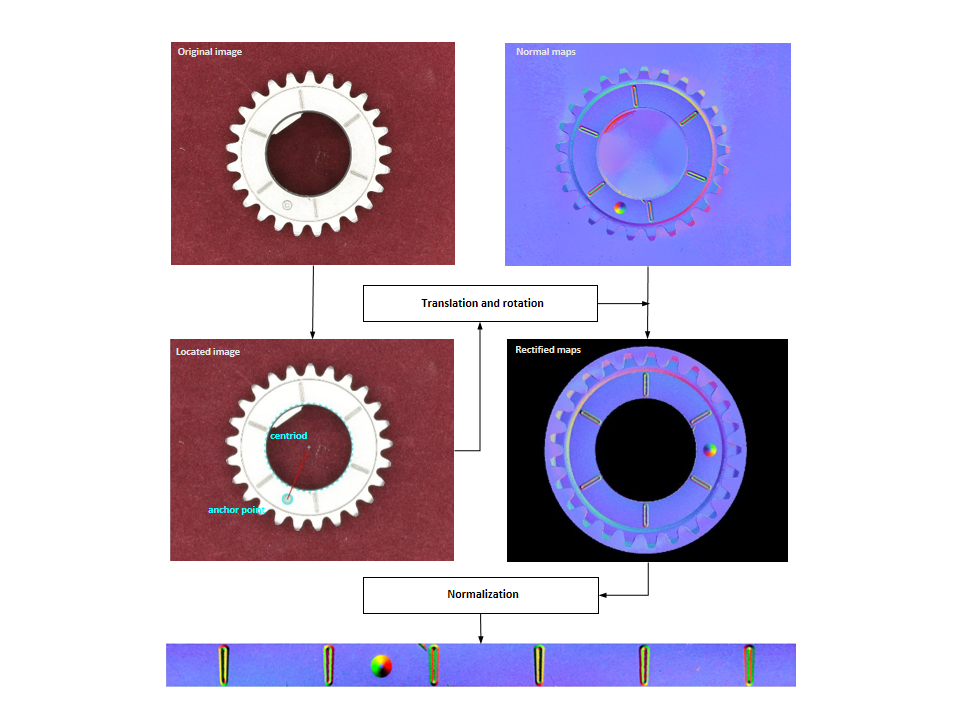
\includegraphics[width=1.0\linewidth]{figures/jiaozhengliuchengtu.png}
\caption{主表面获取结果图}
\label{fig:zhubiaomianhuoquliucheng}
\end{figure}

最大类间方差法又叫做大津法,
该方法假设阈值为${t}^{'}$,
使用${t}^{'}$将图片分为前景(值为1)和背景(值为0)两个区域,
其中属于前景的像素点占图像的比例记为${w}_{0}$,平均灰度值信息记为${u}_{0}$,
背景像素点占图像的比例记为${w}_{1}$,
平均灰度值记为${u}_{1}$,
图像的大小记为
$M\times N$,平均灰度值记为$u$,
类间方差记为$g$,
图像中小于阈值${t}^{'}$
的像素个数记为
${n}_{0}$,大于
${t}^{'}$的像素个数记为
${n}_{1}$,
于是我们可以得到等式\ref{fig:jisuanw0}、\ref{fig:jisuanw1}、\ref{fig:jisuang}。
\begin{gather}
{w}_{0}={n}_{0}/(M\times N) \label{fig:jisuanw0}\\
{w}_{1}={n}_{1}/(M\times N)\label{fig:jisuanw1}\\
g={w}_{0} {({u}_{0}-u)}^{2}+{w}_{1}{(u_1-u)}^{2} \label{fig:jisuang}
\end{gather}
因为灰度值的范围为
$[0-255]$,我们可以使用遍历的方法找到使
$g$最大的
${t}^{'}$,
把这个值作为阈值$b\_t$。

接着我们对生成的二值图像做腐蚀操作,
并去除一些小的连通区域,
然后对其进行膨胀操作,
得到零件和背景分开的二值图像。
在这个二值图像中,
背景被圆环状零件分割成两个部分,
一部分位于圆环中心,
另一部分将零件包裹,
我们首先提取圆环中心部分的质心和半径得到一个内切圆,
接着提取环状零件的圆心和半径,最后提取圆环上的圆形定位点。
结果如图\ref{fig:zhubiaomianhuoquliucheng}所示,
图中$Original image$表示零件照片,
$Normal imgae$表示零件法线图,
$Localted image$表示提取圆心和定位点的结果,
其中蓝色虚线表示提取的圆环中心圆,蓝色实线圆表示零件定位点,红色直线连接了定位点的圆心和圆环中心圆的圆心。
根据提取出来得信息,我们去除掉零件背景区域,
得到圆环状区域$Rectified maps$,
最后我们将环状区域展开成一个矩形,并裁剪掉其边缘部分,得到图\ref{fig:zhubiaomianhuoquliucheng}中最底部显示的零件主表面图。

\subsection{数据增强}
\label{subsection:shujuzengqiang}

首先,随着制造业、冶金业的高速发展,零件的制造工艺不断提高,零件生产过程中缺陷产生的概率变得很小,导致我们拥有的数据量较小,需要使用数据增强的方式扩充数据;
其次,缺陷具有一定旋转不变性,
可以在数据增强阶段体现这一性质。

\subsubsection{分割}
\label{subsubssection:chuantongfenge}

我们首先使用滑动窗口将一张主表面图分割成一组固定大小的图片,
实验过程中,滑动窗口大小固定,
用$WinSize$来表示,
划分后的图片大小和窗口大小相同。
在确定$WinSize$的大小时,
我们遵循两个原则:(1)尽可能使缺陷占图片较大比重;(2)尽可能使图片包含任意单独缺陷。
为了选择合适的$WinSize$,
我们首先人工标记了所有缺陷的
矩形包围盒,这些包围盒的大小用$(w_i,h_i)$表示,
其中$w_i$、$h_i$分别表示第i个包围盒的宽和高,
包围盒宽和高的最大值分别用${w}_{max}$、${h}_{max}$表示,
最小值用${w}_{min}$、、${h}_{min}$表示,
接着我们分别统计了宽和高的直方图,其范围分别为$[{w}_{max},{w}_{min}]$,
$[{h}_{max},{h}_{min}]$,
我们通过观察直方图,确定$WinSize$的大小。
在实验过程中,我们分别尝试过$21*21$、$25*25$、$32*32$、$40*40$
等不同尺寸的窗口,
其中$25*25$的实验效果最理想,为我们最终确定的窗口。
窗口分割结果如图\ref{fig:chuangkoufenge}所示,
$WinSize$为$25*25$,滑动窗口步长为17。
\begin{figure}[htbp]
\centering
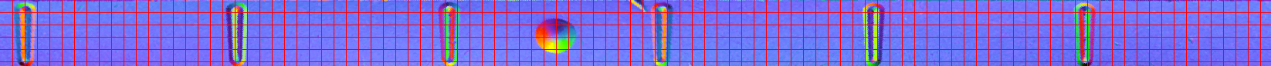
\includegraphics[width=1.0\linewidth]{figures/chuangkoufengetu.png}
\caption{滑动窗口分割示意图}
\label{fig:chuangkoufenge}
\end{figure}

\subsubsection{镜像和旋转}

对于一个有缺陷的零件图片,对其镜像和旋转之后,仍然是一个有缺陷的零件图片,在法线图上也是如此,因此我们可以使用镜像和旋转的方式扩充数据库。
经过分割之后,
所有的数据都变为$25*25$大小的图片,
我们首先对这些图片做镜像,产生新的图片,
接着将所有的图片分别顺时针旋转$45^\circ$、$90^\circ$、$135^\circ$、$180^\circ$、$225^\circ$、$270^\circ$、$315^\circ$,得到新的数据。
镜像和旋转的方法非常简单,可以直接调用opencv\cite{opencv_library}或者matlab\cite{MATLAB:2017}的函数库,本文不再赘述。

\section{特征提取}
\label{section:tezhengtiqu}

本节介绍本文所使用特征提取方法,
这些特征将被用在接下来的模型训练和分类中。

\subsection{Haar-like 特征}

Haar-like特征能反应图像的灰度变化,
最早由Papageorgiou等人提出来应用于人脸检测,
之后Viola和Jones\cite{viola2001rapid}将其扩展为3种类型4种形式。
Haar-like特征的四种形式分为边缘特征、线性特征、中心特征和对角线特征,
特征模板分别如图\ref{fig:haar-like}中$A$、$B$、$C$、$D$所示,
\begin{figure}[htbp]
\centering
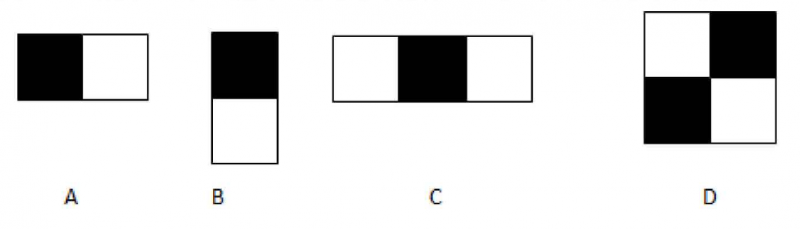
\includegraphics[width=1.0\linewidth]{figures/haarlike.png}
\caption{haar-like特征类型示意图}
\label{fig:haar-like}
\end{figure}
模板内有白色和黑色两种类型的矩形,
模板的特征值为白色矩形内的像素值的和减去黑色矩形内的像素值的和。
提取特征时使用一个滑动窗口,在原始图片中不断移位滑动,
窗口每到一个位置,就计算该窗口区域的特征值。
由于窗口可以位于图像中任意位置,并且窗口大小也可以任意改变,
因此在特征提取过程中会产生非常多的窗口,如果直接计算时间复杂度非常大,
我们可以使用积分图的方法来加速计算,
从而降低特征提取的时间复杂度。

\subsection{图像梯度}
\label{subsection:tidu}

在数学中,梯度(Gradient)是一个具有大小和方向的矢量,在
计算机视觉领域中则把梯度的模简称为梯度。
对于一副图像,我们可以将其看成二维离散函数,图像的梯度就是这个二维离散函数的导数。
和在数学中的意义相似,
图像在梯度值较大的地方,灰度值变化较大,
图像在此处可能存在边缘,在梯度值较小的地方,
灰度值变化较小,图像比较平滑。
数字图像中梯度可以用公式\eqref{eq:g}表示,
其中$dx$表示$x$方向上的梯度,可以用公式\eqref{eq:dx}得到,
$dy$表示$y$方向上的梯度,可以用公式\eqref{eq:dy}得到。
\begin{gather}
G(x,y)=dx(i,j)+dy(i,j)\label{eq:g}\\
dx(i,j)=I(i+1,j)-I(i,j)\label{eq:dx}\\
dy(i,j)=I(i,j+1)-I(i,j)\label{eq:dy}
\end{gather}

在实际求梯度时,更多的是使用差分的方法求导数的近似,
经典的图像梯度算法考虑图像中每个像素某个邻域内的灰度变化,利用边缘近似的一阶或二阶导数变化规律,对原始图像中像素邻域设置梯度算子,用梯度算子计算梯度。
常用的梯度算子有Sobel算子\cite{russ2016image}、Robinson算子\cite{russ2016image}、Laplace算子\cite{russ2016image}等。
本文使用Sobel算子计算图像梯度,
Sobel算子使用两组$3\times 3$的卷积核对图像做卷积操作,
分别求出横向和纵向的梯度近似值,
用$G_x$和$G_y$表示。
假设输入图像为$Image$,
首先将其转换成灰度图,
然后使用Sobel算子的两个卷积核对其卷积,
即可得到$G_x$、$G_y$。
卷积操作如公式\eqref{eq:gx}、\eqref{eq:gy}所示,
\begin{gather}
G_x={S\_Conv}_x*A\label{eq:gx}\\
G_y={S\_Conv}_y*A\label{eq:gy}
\end{gather}
其中,${S\_Conv}_x$表示$x$方向的卷积核,
${S\_Conv}_y$表示$y$方向的卷积核,它们的形式分别如公式\eqref{eq:sconvx}、\eqref{eq:sconvy}所示。
\begin{gather}
{S\_Conv}_x=\begin{bmatrix} -1 & 0 & +1 \\ -2 & 0 & +2\\-1 & 0 & +1\end{bmatrix}  \label{eq:sconvx}\\
{S\_Conv}_y=\begin{bmatrix} +1 & +2 & +1 \\ 0 & 0 & 0\\-1 & -2 & -1\end{bmatrix}  \label{eq:sconvy}
\end{gather}
最终图像的梯度图$G$通过公式\eqref{eq:G}得到。
\begin{equation}
G=\sqrt{G_x^2+G_y^2} \label{eq:G}
\end{equation}
为了提高计算效率,
我们使用公式\eqref{eq:jinsiG}替代\eqref{eq:G}得到$G$的近似解。
\begin{equation}
G= \left| {G}_{y} \right|+ \left| {G}_{y} \right|
\label{eq:jinsiG}
\end{equation}

这一梯度提取算法对噪声具有平滑作用,提取出的梯度特征不仅能够捕捉轮廓信息,还能弱化图像亮度的影响。

\subsection{方向梯度直方图}\label{subsection:tiquzhifangtu}

方向梯度直方图\cite{dalal2005histograms}(HOG)特征最早由法国研究员Dalal在CVPR-2005上提出,
是计算机视觉领域最常用的特征之一,
被广泛应用于物体检测中,并取得了良好的效果。
HOG特征在图像梯度的基础上,
通过统计局部区域的梯度直方图来构成更抽象的特征。

计算时我们需要用到\ref{subsection:tidu}节计算过的
横向梯度$G_x$、
纵向梯度$G_y$
和梯度$G$,
除此之外,我们还需要计算梯度的方向信息。
我们使用角度$\theta$来表示方向,
它可以使用公式\eqref{eq:tidujiaodu}计算得到。
\begin{equation}
\label{eq:tidujiaodu}
\theta (x,y)={\tan^{-1}{\frac{G_x(x,y)}{G_y(x,y)}}}
\end{equation}
接着我们将图像分成若干个单元$(cell)$,
相邻的$cell$之间不重叠,
然后我们统计每个$cell$的方向梯度直方图作为其特征。
在统计时,我们将所有的梯度方向划分为9个$bin$
作为直方图的横轴,
对应范围内梯度值的和作为直方图纵轴,
梯度方向划分方式如图\ref{fig:tiduhuafentu}所示。
\begin{figure}[htbp]
\centering
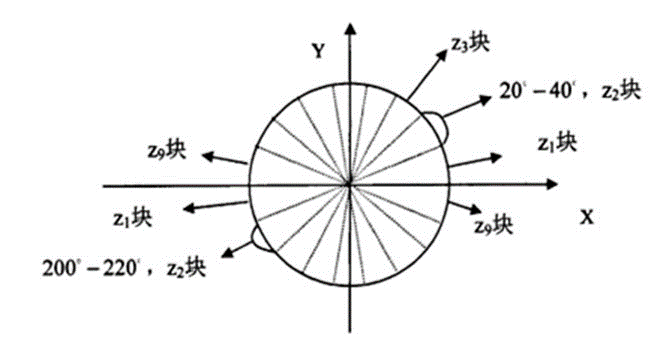
\includegraphics[width=1.0\linewidth]{figures/gradient.png}
\caption{梯度方向划分图}
\label{fig:tiduhuafentu}
\end{figure}
由于局部光照的变化和前背景的变化,
梯度值的范围可能非常大,
因此我们需要对梯度值做归一化。
归一化的方法是把各个$cell$组成空间上连通的区间$(block)$,
$block$的特征为其内部所有$cell$
的特征向量串联的结果,$block$之间可以互相重叠,我们采用滑动窗口来统计每个
$block$的特征,并将它们串联成图片的特征向量。
根据数据的大小,我们设$block$的大小
$blocksize$为
$(10,10)$,设$cell$的大小$cellsize$为
$(5,5)$,
每个$block$
包含四个$cell$。
使用滑动窗口统计$block$的特征时,
滑动窗口的步长$blockstride$设为
$(5,5)$,
这时
$block$之间有重叠,
每一个$cell$的特征都会以不同的结果多次出现在图片的特征向量中。

\subsection{局部二值模式}

局部二值模式$(LBP)$特征是一种常见的图像局部纹理特征,
该特征对光照不敏感,
并且计算方法简单,数据量小,是一种非常实用的特征。
原始的LBP算子由T. Ojala, M.Pietikäinen和 D. Harwood提出,
该算子使用像素点的$3\times 3$邻域求LBP特征。
随后Ojala等人提出了圆形LBP算子\cite{ojala2002multiresolution},将原始算子的$3\times 3$邻域扩展到任意领域,
并使其获得了灰度不变性和旋转不变性,
Ojala还提出采用“等价模式”\cite{ojala2002multiresolution}对LBP算子降维,
使得特征在减少维度的情况下仍能较好的代表图像局部纹理。

我们将LBP算子定义在
$3\times 3$的窗口内,
将窗口中心像素灰度值记为阈值$l\_thre$,接着我们将其与周围相邻的8个像素的灰度值比较,
若周围像素点的灰度值大于$l\_thre$,那么该点的位置被标记为1,
否则被标记为0,
最终中心像素点$3\times 3$
邻域内的8个点产生8个0或者1,我们将其从左上角位置开始顺时针排列成一个二进制数,将这个二进制数的大小当做中心像素点的LBP特征值,
如图\ref{fig:lbp}所示。
\begin{figure}[htbp]
\centering
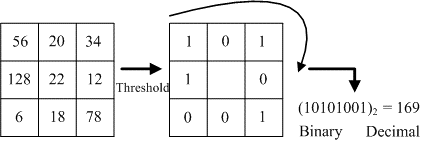
\includegraphics[width=1.0\linewidth]{figures/lbp.png}
\caption{LBP特征提取示意图}
\label{fig:lbp}
\end{figure}
从图\ref{fig:lbp}中可以看出,LBP特征的二进制数是以一定顺序编码得到的,如果图像发生旋转,其值就会发生改变,为此我们主动旋转其邻域,得到一系列LBP值,取其最小值作为最终LBP值,旋转过程如图\ref{fig:lbp2},这种方法得到的特征值拥有良好的旋转不变性。
\begin{figure}[htbp]
\centering
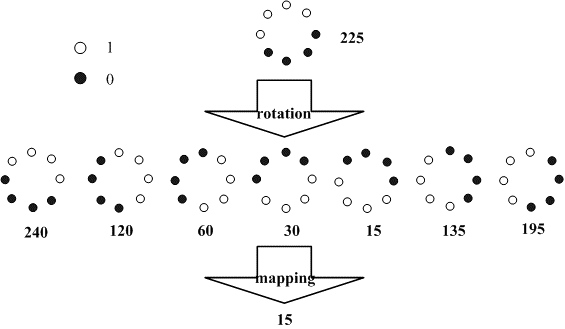
\includegraphics[width=1.0\linewidth]{figures/lbp2.png}
\caption{LBP旋转不变性示意图}
\label{fig:lbp2}
\end{figure}

接着,我们观察LBP值中从$0\rightarrow 1$或从$1\rightarrow 0$的跳变次数,
如果最多只有两次跳变,
则认为这个LBP值所对应的二进制是一个等价模式,
保留这个LBP值,否则将其划分到混合模式类,
所有混合模式类使用同一个LBP值。
最终,每个像素点都得到一个LBP值,我们并不直接使用这个值,
而是使用滑动窗口的方式获得窗口内LBP值的直方图,
将直方图作为窗口的特征,
最后将所有窗口的特征串联起来,得到整幅图像的特征。
本文实验中,滑动窗口的大小和步长和HOG特征中$block$的大小和步长相等。

\subsection{灰度共生矩阵}

灰度共生矩阵特征首先得到图像的共生矩阵,
然后通过计算该共生矩阵得到矩阵的特征值,
用这些特征值来代表图像的纹理特征。
灰度共生矩阵能够反映图像灰度方向、相邻间隔、变化幅度等综合信息。

灰度共生矩阵特征建立在图像灰度图的基础上,
因此我们首先将图片转换成灰度图$Gray$,
接着统计其灰度共生矩阵。
统计灰度共生矩阵时,我们首先取图像中任意一个点
$(x,y)$,
其灰度值记为${g}_{1}$,
取图像中另外一个点$(x+a,y+b)$,
其灰度值记为${g}_{2}$,
可以得到一个灰度值对$({g}_{1},{g}_{2})$,
当$a$、$b$固定不变,
对图像中所有的点$({x}^{'},{y}^{'})$
找对应的$({x}^{'}+a,{y}^{'}+b)$,
都可以得到一个灰度值对$({g}_{1}^{'},{g}_{2}^{'})$,
接着我们统计所有灰度值对中相同$({g}_{1}^{'},{g}_{2}^{'})$
出现的次数,
将它们排列成一个方阵,
这个方阵就是灰度共生矩阵,
方阵中在$({g}_{1},{g}_{2})$位置
上的值为$({g}_{1},{g}_{2})$出现的概率$p({g}_{1},{g}_{2})$,
$(a,b)$被称为距离差分值,
常采用不同的组合以得到不同的灰度共生矩阵,
本文使用$(1,0)$、$(0,1)$、$(1,1)$、$(-1,-1)$
作为$(a,b)$的选择,
分别对应对图片进行${0}^{\circ}$、${90}^{\circ}$、${45}^{\circ}$、${135}^{\circ}$的扫描结果。

\subsection{色彩空间}

除了传统的图像特征以外,
我们还分析了法线图色彩空间的特点。
我们将法线图记为$Normal$,
将其大小记为$M*N$,
我们用$M$表示图像宽度$width$的大小,沿着宽从左到右的方向记为水平方向,
用$N$表示图像高度$Height$的大小,沿着高从低到高的方向记为垂直方向。
首先,我们对法线图三个通道的像素值
分别在垂直和水平方向上进行投影,观察不同的投影结果。
在水平方向上的投影可以用公式
\eqref{eq:chuizhitouying}表示,
\begin{equation}
p_i=\sum_{j=0}^{N-1} I(i,j),\qquad i\in \left[ 0,M-1\right]
\label{eq:chuizhitouying}
\end{equation}
其中$p_i$表示在水平方向i点上的投影值,
$I(i,j)$表示图像中$(i,j)$位置的像素值。
接着我们对$p_i$进行归一化,
使$p_i$的值都处于$[0,1.0]$的范围内。
我们对图像在垂直方向上也做了同样的投影,
并在$B$通道水平投影上发现了明显的统计规律。如图\ref{fig:secaitongying}所示,
\begin{figure}[htbp]
\centering
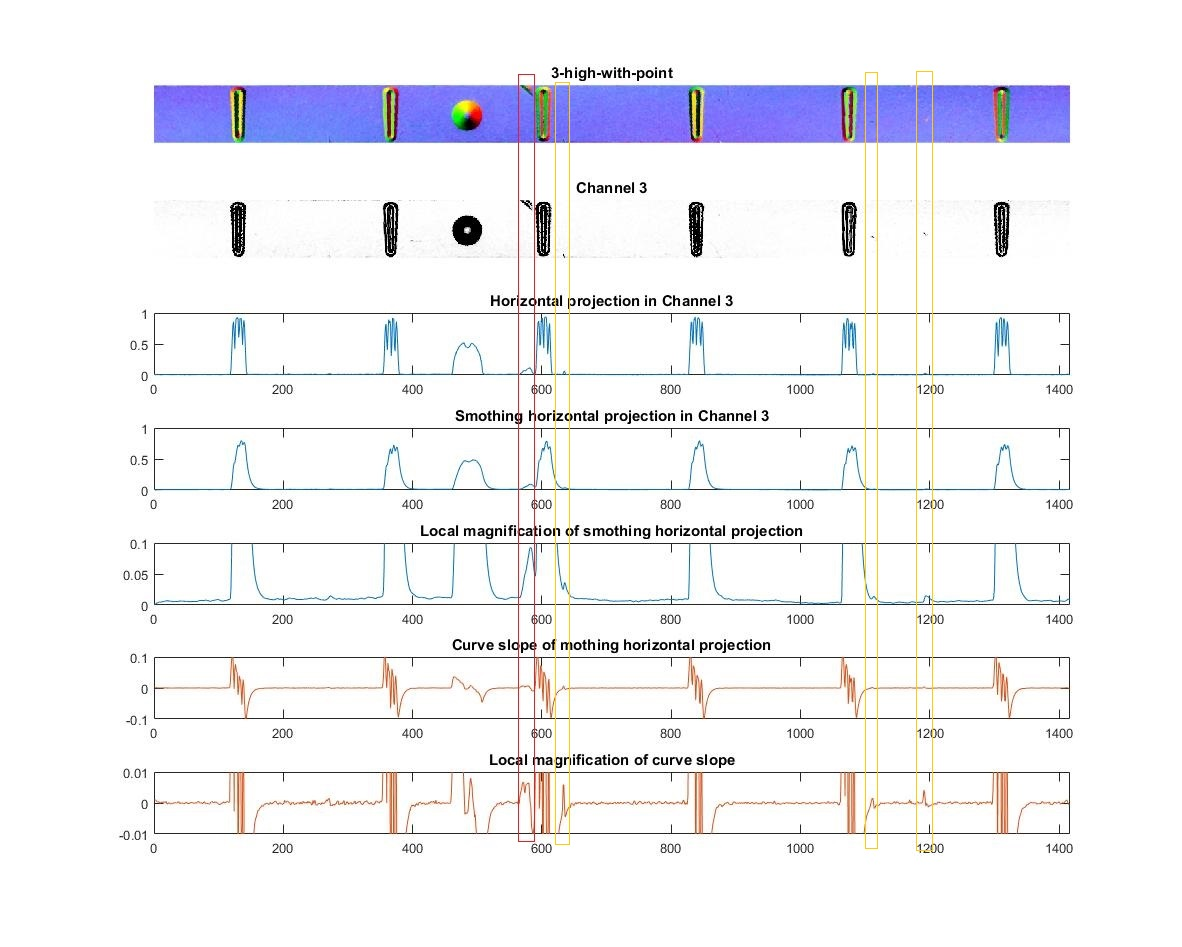
\includegraphics[width=1.0\linewidth]{figures/secaikongjian.png}
\caption{水平投影结果图}
\label{fig:secaitongying}
\end{figure}
图中$3-high-with-point$表示零件法线图,
$channel~3$表示法线图$B$通道信息,
$Horizontal~projection~in~Channel~3$表示$channel~3$水平投影的归一化结果,
$Smothing~horizontal~projection~in~Channel~3$表示对水平投影平滑后的结果,
$Local~mangnification~of~smothing~horizontal$表示平滑后的水平投影在
$[0.0,0.1]$范围内的结果,
$Curve~slope~of~smoothing~horizontal~projection$
表示平滑后水平投影的导数信息,
$Local~magnification~of~curve~slope$表示导数在$[-0.01,0.01]$范围内的结果,
红色矩形框表示零件缺陷区域,
黄色矩形框表示零件中的划痕、凹陷等区域,这些划痕、凹陷太小不足以构成缺陷。
从图中可以明显看出,在有缺陷的区域,投影值会产生剧烈抖动,
而在没有缺陷的区域,投影值非常平滑,
因此我们直接将法线图的色彩信息作为图像的一种特征。

\section{分类器设计、训练和检测}


本文使用支持向量机作为基分类器,
利用Adaboost的方法将不同的基分类器组合成一个强分类器。
在训练阶段,考虑到数据不平衡的问题,我们将数据集划分成不同的子数据集,
对于每一个子数据集训练一个强分类器,
在检测阶段,我们将不同子集训练出来的强分类器组合成一个级联检测器,
使用级联检测器进行缺陷检测。
本节首先介绍支持向量机的相关概念以及如何对其进行训练,之后介绍如何使用Adaboost将其组合成一个强分类器,最后介绍如何用级联的方法将不同的强分类器组合成级联检测器。

\subsection{支持向量机}
\label{subsection:svm}

分类一直是机器学习中非常基础和重要的领域,
常见的分类模型有随机森林\cite{breiman2001random}(Random Forest,简称 RF)、
对数几率回归\cite{周志华2016机器学习}(Logistic Regression,简称 LR)、
贝叶斯分类器以及支持向量机(SVM)等。
其中,支持向量机作为一种基于统计学习理论的监督学习算法,能在样本数量较少的情况下学习出一个不错的分类决策,
并且可以使用核函数的方法解决高维问题,
处理非线性特征的相互作用,
SVM无需依赖全部数据集,具有良好的泛化能力。
基于本文数据量小、特征维度高、线性不可分等特点,我们选择SVM作为基分类模型。

首先,
我们使用$D$来表示数据集,
并将$D$中的样本分为两类,一类是有缺陷的样本,
标记为$+1$,
一类为没有缺陷的样本,标记为$-1$,
那么$D$可以用公式\eqref{eq:shujujid}来表示,其中$x$表示样本的特征向量,$y$表示样本的标记。
\begin{equation}
\centering
D={(x_1,y_1), 
(x_2,y_2),…,(x_m,y_m)},\quad y_i\in \{-1,+1\}
\label{eq:shujujid}
\end{equation}
支持向量机通过在特征空间中构建一个超平面来划分不同的类别,
这个超平面就是这两个类的分类边界。
在特征空间中,使用公式\eqref{eq:svmgongshi}来描述这个超平面,
\begin{equation}
\centering
w^Tx+b=0
\label{eq:svmgongshi}
\end{equation}
公式中,
$x$表示特征向量,
$w=(w_1;w_2;…;w_d)$表示分类超平面的法向量,决定了超平面的方向,
$b$表示超平面的位移向量,决定了超平面到原点的距离,
根据$W$和$b$
可以唯一确定一个超平面$(w,b)$。
特征空间中点$x$到超平面$(w,b)$的距离$r$用公式\eqref{eq:r}表示,
观察该公式不难发现,$r$的大小可以通过改变$w$和$b$的值而改变。
\begin{equation}
\centering
r=\frac{\left| w^Tx+b\right|}{\lVert w\rVert}
\label{eq:r}
\end{equation}
假设超平面$(W,b)$可以将样本正确分类,
那么对于任意$(x_i,y_i)\in D$,若$y_i=+1$,则$w^T x_i+b>0$,若$y_i=-1$,则$w^T x_i+b<0$,这一条件可以用公式\eqref{eq:fenleigongshi}表示。
\begin{equation}
\centering
\begin{cases}
w^Tx_i+b>+1 ,\quad y_i=+1\\
w^Tx_i+b<-1 ,\quad y_i=-1
\end{cases}
\label{eq:fenleigongshi}
\end{equation}
并且如图\ref{fig:svm}所示,
公式\eqref{eq:fenleigongshi}中能使等号成立的点恰好是距离超平面最近的特征点,
它们被称为“支持向量”,
两个不同类支持向量到超平面的距离之和$\gamma$被称为间隔,可以用公式\eqref{eq:jiange}表示。
\begin{equation}
\centering
\gamma = \frac{2}{ \lVert w\rVert }
\label{eq:jiange}
\end{equation}
\begin{figure}[htbp]
\centering
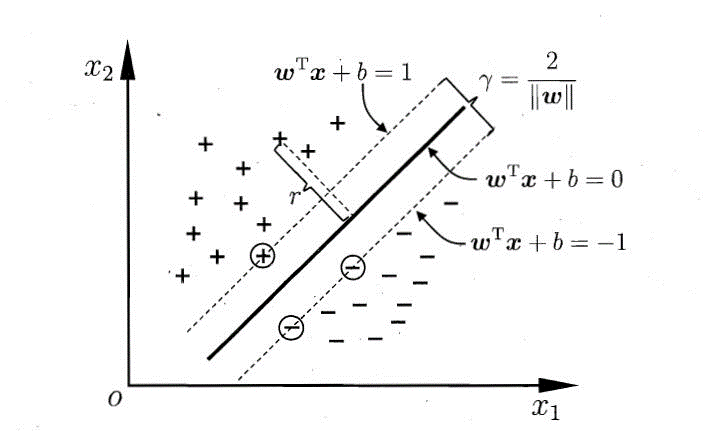
\includegraphics[width=1.0\linewidth]{figures/svm.png}
\caption{支持向量机示意图}
\label{fig:svm}
\end{figure}
SVM的核心思想是找到一个具有最大间隔的超平面,
即找到满足约束\eqref{eq:fenleigongshi}并使得$\gamma$最大的参数$w$和$b$,
可以用公式\eqref{eq:svmyueshutiaojian}表示这一约束条件。
\begin{equation}
\centering
\begin{aligned}
&\ \max_{w,b}{\frac{2}{\lVert w\rVert}}\\
&\ \mbox{s.t.}\quad y_i(w^Tx_i+b)\ge 1, \quad i=1,2,\cdots ,m.
\end{aligned}
\label{eq:svmyueshutiaojian}
\end{equation}
观察上式,为了最大化间隔,
只需要最大化${\lVert w\rVert}^{-1}$,
这等价于最小化${\lVert w\rVert}^2$,
于是我们可以将公式\eqref{eq:svmyueshutiaojian}改写为公式\eqref{eq:svmyueshutiaojian1}的形式。
\begin{equation}
\centering
\begin{aligned}
&\ \max_{w,b}{\frac{1}{2}\lVert w\rVert^2}\\
&\ \mbox{s.t.}\quad y_i(w^Tx_i+b)\ge 1,\quad i=1,2,\cdots ,m.
\end{aligned}
\label{eq:svmyueshutiaojian1}
\end{equation}
这是一个凸优化二次规划问题,
可以直接用现成的优化包求解。

虽然我们希望超平面能够将两个类完全分开,
但是现实任务中往往很难找到这样的超平面,
并且就算找到了这样的超平面,也很难判断这是不是过拟合导致的。
为了解决这一问题,我们允许某些样本不满足约束条件,只是要求不满足约束的样本尽可能少,这种方法被称为“软间隔”,它的优化目标可以用公式\eqref{eq:svmyouhuayueshu}表示,
\begin{equation}
\centering
\min_{w,b}{\frac{1}{2}\lVert w\rVert^2}+C\sum_{i=1}^{m}{y_i(w^Tx_i+b)-1}
\label{eq:svmyouhuayueshu}
\end{equation}
其中$C$是一个大于0常数,被称为正则化常数,
它需要人工优化,后面会讲到如何优化它,
$l_{0/1}$表示“$0/1$损失函数”,由于其非凸、非连续的性质,不易直接求解,实际使用时常用其他函数替代,本文使用hinge损失函数替代。

\subsection{核函数}

\ref{subsection:svm}节中描述了基本的SVM模型,
这一模型假设两个类在特征空间中线性可分,
然而在实际情况中,样本在特征空间中往往是线性不可分的。
为了解决特征空间线性不可分的问题,
SVM使用核函数的方法将数据从特征空间映射到高维空间中,
在高维空间中寻找一个可以将两个类分开的超平面。

对于原始特征空间中特征向量$x$,令$\phi(x)$表示将$x$映射到高维空间中的特征向量,
我们可以得到高维空间中对应的SVM模型,如公式
\eqref{eq:chaopingmian}所示,
\begin{equation}
\centering
f(x)=w^T\phi (x)+b 
\label{eq:chaopingmian}
\end{equation}
其中,$w$和$b$表示需要求解的模型参数,
类似于\ref{subsection:svm}中的SVM最优化形式,
这一公式的最优化形式可以用公式\eqref{eq:svmyueshutiaojian2}表示。
\begin{equation}
\centering
\begin{aligned}
&\ \min_{w,b}{\frac{1}{2}\lVert w\rVert^2}\\
&\ \mbox{s.t.} \quad y_i(w^T\phi (x_i)+b)\ge 1,\quad i=1,2,\cdots ,m.
\end{aligned}
\label{eq:svmyueshutiaojian2}
\end{equation}
求解该问题涉及到计算特征向量$x_i$和$x_j$
在高维空间中的內积${\phi (x_i)}^T \phi(x_j)$。
由于我们要将原始特征空间映射到高维空间甚至无穷维空间中,
因此直接计算${\phi (x_i)}^T \phi(x_j)$往往非常困难,
“核函数”正是为了解决这个问题,
核函数$k(.,.)$
具有如公式\eqref{eq:hehanshuxingzhi}所示的性质。
\begin{equation}
\centering
k(x_i,x_j )=\langle \phi (x_i ),\phi (x_j )\rangle=\phi (x_i )^T \phi (x_j )
\label{eq:hehanshuxingzhi}
\end{equation}
使用核函数,可以通过$x_i$和$x_j$在原始样本空间中的內积
得到其在高维空间中的內积,
使得我们可以避免直接计算高维甚至无穷维特征空间中的內积。
常用的核函数有线性核函数、多项式核函数、卡方核函数、高斯核函数、拉普拉斯核函数以及
$Sigmoid$核函数。

本文SVM算法基于libsvm\cite{CC01a}库实现,该库中预定义了很多基本核函数,可以很方便的使用。在实验中,我们测试了不同的核函数在数据集上的表现,其中高斯核表现最好也最稳定,因此,本文使用高斯核将原始特征空间映射到高维空间。
\begin{equation}
\centering
k(x_i,x_j )=\exp {⁡(-\frac{\lVert x_i-x_j \rVert ^2}{2\sigma ^2 })}
\label{eq:gaosihe}
\end{equation}

高斯核的基本形式如公式\eqref{eq:gaosihe}所示,
其中,$\sigma$表示高斯核的带宽,
是一个大于0的数,
也是使用高斯核函数时需要调整的参数。

\subsection{支持向量机训练}

在训练SVM模型时,需要人工设定的超参数有正则化常数$C$和
高斯核函数的带宽$\sigma$。
在实际训练时,
我们并不直接设定$C$和$\sigma$的值,
而是通过一定的方法来选择不同的参数,
并使用交叉验证的方法验证参数的效果,
最终使用效果最好的参数作为超参训练模型。

模型中$C$和$\sigma$是相互独立的,因此二者可以独立选择。
我们首先从$[-10,15]$中选择$\log_2⁡C$的值,
从$[-20,5]$中$\log_2⁡\sigma$的值,
然后用这组值$(C,\sigma)$作为超参训练模型,
并使用交叉验证法对模型评估,
不断重复这一过程,尝试不同的组合,
选择评估结果最好的$(C,\sigma)$作为最终的模型参数。

交叉验证法首先将原始数据集$D$划分为$K$个大小相似的互斥子集,
即$D=D_1\bigcup D_2\bigcup \dots \bigcup D_k,\quad D_i\bigcap D_j=\varnothing \quad(i\not =j)$,
本文实验中$K$取$5$,
每个子集从$D$中分层采样得到,
接着我们分别用第$k$个子集作为测试集,
用余下$k-1$个子集的并集作为训练集,
对模型进行训练和评估,
得到$k$个评估结果,
使用这$k$个评估结果的均值来评价参数的好坏。

\subsection{自适应增强算法}
\label{subsection:adaboost}

自适应增强算法(Adaboost)是boosting族算法中最具代表性的算法,
本文用它将不同的SVM模型组合成一个强分类模型。
Adaboost算法可以组合多个基学习器,
它首先训练一个基学习器,根据基学习器的表现对样本权重进行调整,
使该学习器中分类错误的样本权重更高,
然后基于调整后的样本训练下一个基学习器,
重复上述步骤直到学习器数目达到指定的值$T$,
最后将这$T$个学习器进行加权组合。

Adaboost可以用“加性模型”表示,如公式\eqref{eq:adaboostjiaxingmoxing}所示,
其中$H(x)$表示模型的最终输出,
$h_t (x)$表示基学习器的输出,
$\alpha_t$表示基学习器的权重。
Adaboost通过最小化指数损失函数优化基学习器的权重$\alpha_t$。
Adaboost在获得$H_{t-1}$之后调整样本权重,
样本权重调整的目标是使下一个基学习器$h_t$能够纠正$H_{t-1}$的错误。
\begin{equation}
H(x)=\sum_{t=1}^T{\alpha_th_t(x)}
\label{eq:adaboostjiaxingmoxing}
\end{equation}

我们使用SVM作为Adaboost的基学习器,假设第$t$个模型$h_t$的分类误差为$\varepsilon_t=1/N\left[\sum_jw_j\delta(h(x_j)\not =y_j)\right]$,
其中,$N$表示样本的数量,
$w$表示样本的权重,
那么模型权重和样本权重的更新公式
可以分别用\eqref{eq:adaboostquanzhigengxin}和\eqref{eq:adaviistshujujiquanzhigengxin}表示,
其中$D_{t}(i)$表示每个样本的权重,
$Z_t$表示使$D_t(i)$符合一个分布的归一化常数。
\begin{gather}
\alpha_t=\frac{1}{2}\ln \frac{1-\varepsilon_t}{\varepsilon_t}  \label{eq:adaboostquanzhigengxin}\\
D_{t+1}(i)=\frac{D_t(i)}{Z_t}\times
\begin{cases}
 ~~e^{-\alpha_t},\quad &\mbox{if}~~h(x_j)=y_i\\
 ~~e^{\alpha_t},\quad &\mbox{otherwise} 
\end{cases}\label{eq:adaviistshujujiquanzhigengxin}
\end{gather}

通过Adaboost训练出来的强分类器会对每个样本输出一个值$p$,
它可以被看做该样本是否为正样本的概率,
我们可以设置一个阈值$threshold$,
当$p>threshold$时,认为该样本为正样本,
也就是该样本有缺陷,
当$p\leq threshold$时,认为该样本为负样本。
显然,如果我们设置的$threshold$较高,模型会有更低的误识率,但是它的检测率也会变低,
如果我们设置的$threshold$较低,检测率会变高,但是误识率也会随之提高,这一问题可以通过增加强分类器个数,使用级联的方式做检测的方法进行优化。

\subsection{级联检测器}
\label{subsection:jilianjianceqi}

在实验过程中,
人工标记的正样本集$P$(有缺陷的样本的集合)
是小于负样本集N(没有缺陷的样本集合)的,
尤其是经过数据增强之后,样本不平衡的问题更加突出。
因此,在训练模型的时候我们并非直接使用全部训练样本训练模型,
而是将负样本分成K个子集$\{N_1,N_1,\dots,N_k\}$,这些子集的大小与$P$相同,
K是由P和N的大小确定的,取$K=ceil(|N|/|P|)$,
$|N|$表示集合$N$的元素个数,
$|P|$表示集合$P$的元素个数,
$ceil()$表示向上取整函数。
子集的划分使用随机抽样的方法,
如图所示,
我们首先从$N$中随机无放回的抽取$|P|$个元素组成第一个子集$N_1$,
接着不断重复这一过程直到得到$k-1$个子集,
这时$N$中剩余的元素个数为$N_{rmain}$,
我们从得到的$k-1$个子集中随机的抽取$|P|-N_{rmain}$个元素,
将这些元素和$N$中剩余的元素组成第K个子集。
我们分别将这$K$个子集和正样本集$P$组成一组子数据集,
从而得到$k$个正负样本均衡的子数据集。
对于每个子数据集,我们训练一个强分类器,
最后使用级联\cite{viola2001rapid}(Cascade)的方式将这些分类器用于缺陷检测。
\begin{figure}[htbp]
\centering
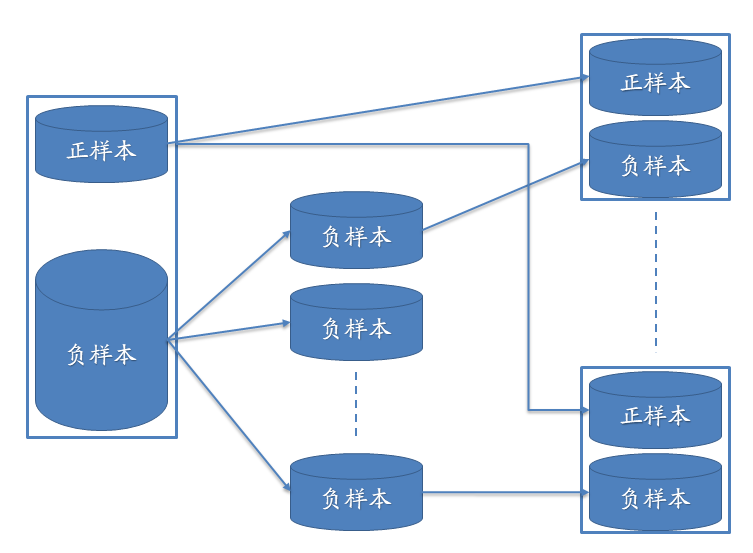
\includegraphics[width=0.8\linewidth]{figures/db.png}
\caption{数据集划分型图}
\label{fig:cascade}
\end{figure}

级联分类器流程如图\ref{fig:cascade}所示,首先使用Adaboost组合SVM训练出$K$个不同的强分类器,
我们将每个强分类器的检测视作一个$stage$,每个$stage$中基分类器的个数为$n$。
在检测的时候使用滑动窗口的方式将输入图片划分成不同的窗口,首先将所有的窗口用第一个强分类器进行分类,即用$stage~1$分类,
将所有检测为正常的窗口归到$Reject~sub-windows$中,
认为这些窗口为正常零件,
将所有检测为缺陷的窗口送往下一个$stage$中,
重复这一步骤,
直到所有的强分类器都检测这一窗口为缺陷,将其视为缺陷,归入$targets$中。
\begin{figure}[htbp]
\centering
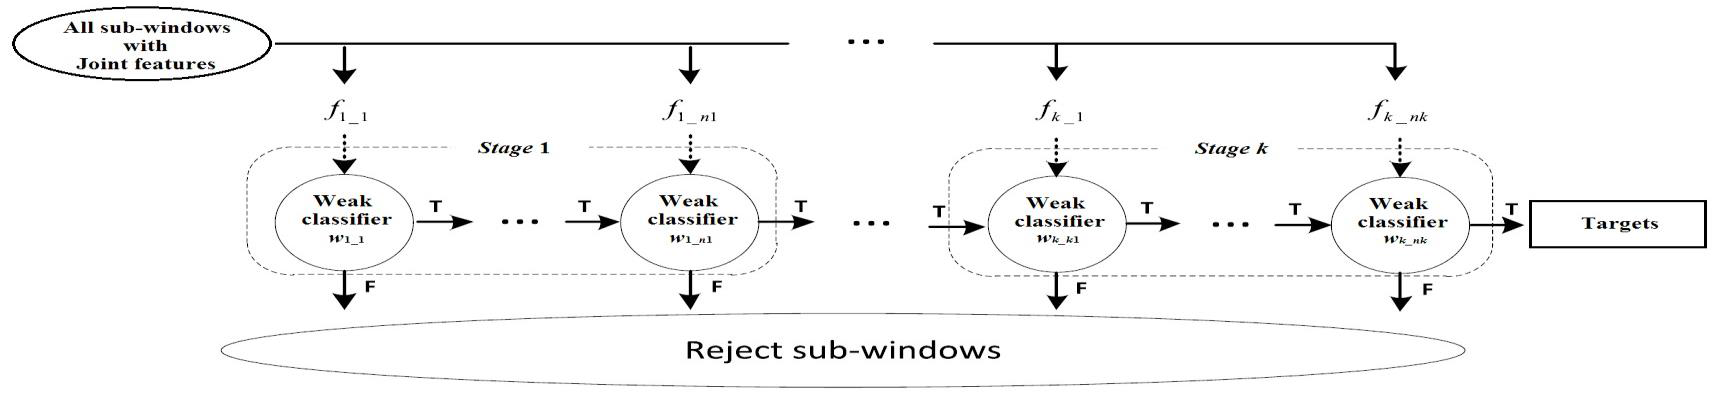
\includegraphics[width=1.0\linewidth]{figures/cascade.png}
\caption{级联分类器模型图}
\label{fig:cascade}
\end{figure}

由于在缺陷检测中,一旦发生漏检,缺陷零件流出,往往会造成重大损失,
相对于漏检,误检一个、几个甚至几十个零件所带来的损失往往可以忽略不计,我们需要尽可能的提高检测率,在检测率尽可能高的情况下降低误识率。
我们在选择强分类器阈值时,选择能使模型达到最大检测率的最大值。


\section{实验结果和分析}
\label{section:shiyanjieguo}

本节首先描述实验环境,然后描述实验过程和实验结果。实验结果主要包括两个部分,
第一个部分为特征提取结果,
第二个部分为缺陷检测结果。

\subsection{实验环境}

实验环境为一台拥有$\mbox{Intel Core}
~I7-7700$处理器的计算机,
该机器的系统为$Win7$,
处理器内存为$8GB$。
本文使用的语言主要有matlab\cite{MATLAB:2017}、C++、python等。
用到的库主要有matlab\cite{MATLAB:2017}、OpenCV\cite{opencv_library}、libsvm\cite{CC01a}等。

\subsection{特征提取结果}

我们使用\ref{section:tezhengtiqu}节中介绍的特征提取方法对数据进行特征提取。
在特征提取过程中,
我们并不是在分割后的图片上提取,
而是先提取整幅图片的特征,
再使用滑动窗口的方法得到分割图片的特征,这种算法大大加速了整个计算流程。

以梯度特征为例,我们首先计算整幅图像的梯度,
用矩阵的形式保存梯度信息,
图片大小用$N\times M$表示,图像中的像素点位置用$(x,y)$表示,
保存梯度信息的矩阵大小为$N\times M$,
矩阵中$(x,y)$位置的值代表了对应图片$(x,y)$位置的梯度信息,
在使用滑动窗口对主表面图进行分割时,只需要选取对应窗口的梯度信息,
即可得到分割后图片的梯度特征。

我们选择一组数据为例介绍特征提取结果。如图\ref{fig:butogndengguangzhankaitu}所示为该组数据在不同光照条件下拍摄的照片和法线图,
其中$Top$为顶部光源照射时的拍摄照片,可以看到由于金属零件表面高光的原因,照片中只有特别明显的缺陷和划痕才能看到,细节部分被完全掩盖了;
$East$、$West$、$South$、$North$分别代表了东部灯光组、西部灯光组、南部灯光组和北部灯光组亮照射时的照片,
这些照片色彩丰富,纹理清晰,
拥有丰富的细节,即是非常微小的纹理、裂缝、划痕、污点也不会丢失,
这些丰富的细节虽然提供了大量信息,但其中干扰信息过多,无疑增大了缺陷检测的难度;
$Normal$表示法线主表面图,
该图能够很好地滤除无用纹理和色彩信息,同时保留由裂缝、划痕等缺陷造成的表面信息。

\begin{figure}[htbp]
\centering
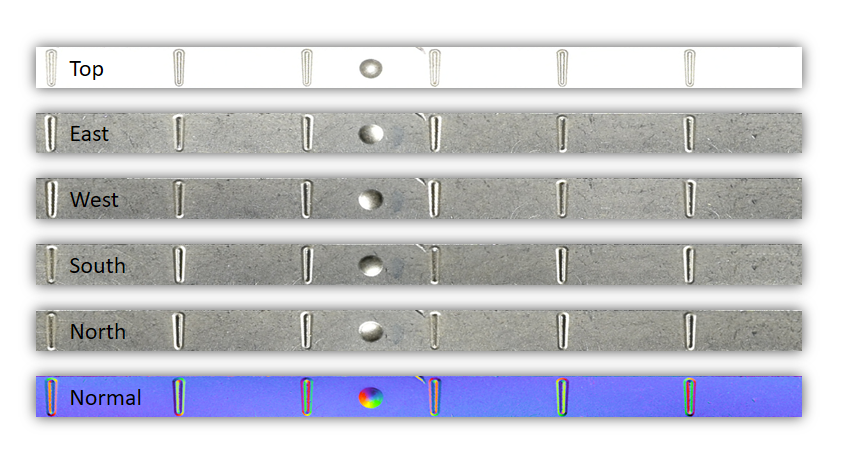
\includegraphics[width=1.0\linewidth]{figures/butongdengguangzhankaitu.png}
\caption{不同光照下主表面结果图}
\label{fig:butogndengguangzhankaitu}
\end{figure}

为了进一步对比不同数据对分类的影响,
我们使用canny\cite{canny1983finding}算子提取它们的边缘信息。
canny算子在提取边缘信息的时候,
需要设定两个滞后性阈值$threshold1$和$threshold2$,
其中二者的较小值的被用于边缘连接,较大值被用来控制强边缘的初始段,
我们将两个阈值分别设为$100$和$300$,同时设定canny算子中sobel算子的卷积核大小为$3$。
\begin{figure}[htbp]
\centering
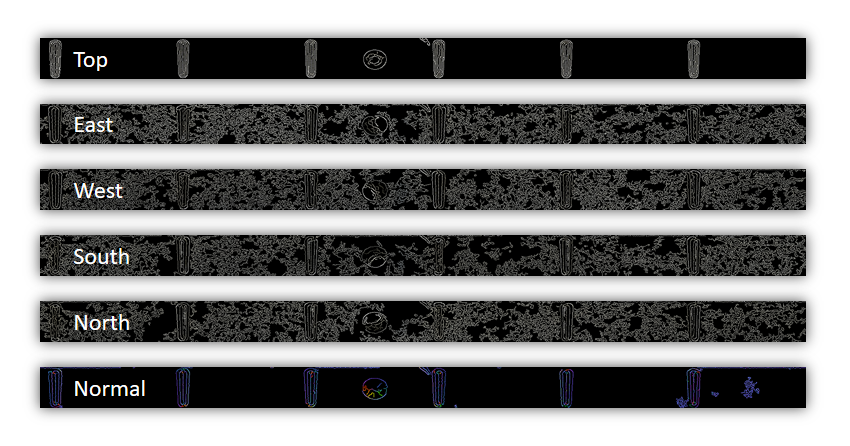
\includegraphics[width=1.0\linewidth]{figures/butongdengguangcanny.png}
\caption{不同光照下边缘检测结果图}
\label{fig:butongdengguangcanny}
\end{figure}
得到的结果如图\ref{fig:butongdengguangcanny}所示,
该组图的命名规则和图\ref{fig:butogndengguangzhankaitu}一样。
从边缘提取图片中的边缘密度可以看出,
$Top$和$Normal$边缘相对简单,和真正的边缘比较接近,
但是$Top$中边缘信息太少,有些缺陷的边缘甚至没有被提取出来,
而$Normal$中没有这个问题;
不同方向光源下的照片边缘过多,这些边缘大多由图片的色彩、纹理等造成,和缺陷检测无关。


\begin{figure}[htbp]
\centering
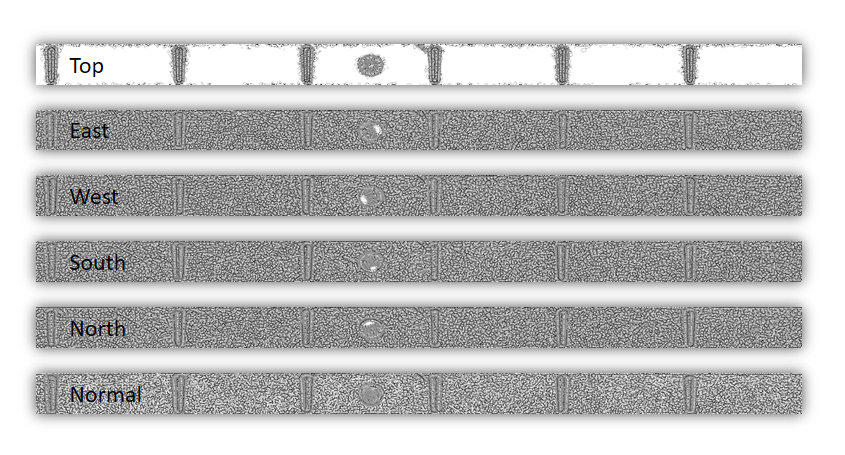
\includegraphics[width=1.0\linewidth]{figures/butongdengguanglbp.png}
\caption{不同光照下LBP特征提取结果图}
\label{fig:butongdengguanglbp}
\end{figure}
\begin{figure}[htbp]
\centering
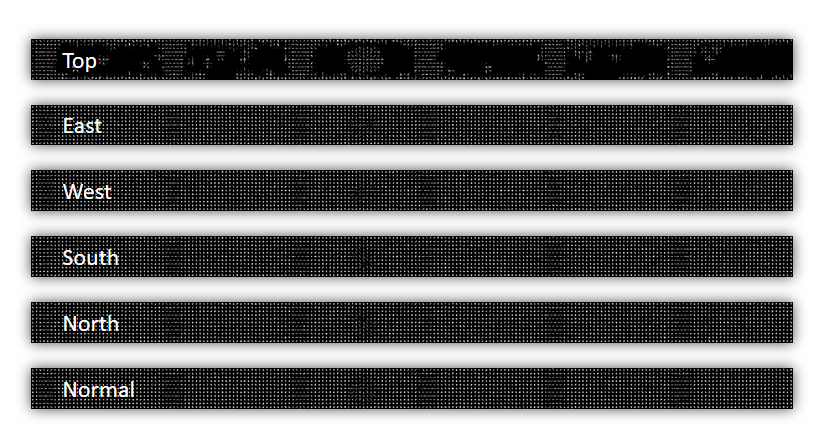
\includegraphics[width=1.0\linewidth]{figures/butongengguanghog.png}
\caption{不同光照下HOG特征提取结果图}
\label{fig:butongengguanghog}
\end{figure}

上述特点还体现在其它特征提取结果中。
如图\ref{fig:butongdengguanglbp}
和图\ref{fig:butongengguanghog}分别展示了提取LBP特征和HOG特征的结果,
由于$Top$过滤掉了太多信息,无论是LBP特征还是HOG特征都会出现大量空白,甚至在有缺陷的地方也出现空白;而不同方向光源下照片的特征提取结果则过于密集,没有明显规律;
法线图的特征提取结果则综合了二者的优点,具有良好的性质。

\subsection{缺陷检测结果}
\label{subsection:chuantongjiancejieguo}

本文使用召回率($recall$,记为$REC$)、
查准率($precision$,记为$PRE$)、
漏检率( $missing~detection~rate$,记为$MDR$)、
误检率($false~detection~rate$,记为$FDR$)
作为模型评价标准,
其中召回率和漏检率是最重要的标准,误检率往往不是特别重要。
假设总共用来测试的零件数量为$N$,
其中正样本即有缺陷的样本数量为$N_p$,
负样本即没有缺陷的样本个数为$N_n$,
显然有$N=N_p+N_n$。其中,$N_p$个正样本中分类正确的个数为$TP$,
分类错误的个数为$FN$,
$N_n$个负样本中分类正确的个数为$TN$,
分类错误的个数为$FP$。
我们可以使用公式\eqref{eq:rec}、\eqref{eq:pre}、\eqref{eq:mdr}、\eqref{eq:fdr}
计算评估指标,显然有$MDR=1-REC$。
\begin{gather}
REC=\frac{TP}{TP+FN}\label{eq:rec}\\
PRE=\frac{TP}{TP+FP}\label{eq:pre}\\
MDR=\frac{FN}{TP+FN}\label{eq:mdr}\\
FDR=\frac{FP}{FP+TN}\label{eq:fdr}
\end{gather}

经过数据预处理之后,我们得到1128张有缺陷的正样本图片和6328张无缺陷的负样本图片,
接着我们将其划分为7个子数据集,每个数据集中各包含1128个正样本和1128个负样本。
我们首先选择一个子数据集,
在这个子数据集上,
分别使用不同灯光条件下的照片和法线图的
HOG特征作为输入,训练一个强分类器,
并设置阈值为0.9来分类。
典型分类结果如图\ref{fig:chuantongjiancejieguo}所示,
其中黄色矩形标出了检测为缺陷的窗口,
$(c)$、$(d)$、$(e)$、$(f)$
分别表示东、西、南、北四组光照图片的检测结果。因为南、北和东、西两组结果非常相似,
因此我们分别展示两组数据的结果,一组零件包含两个缺陷,结果为图中$(c)$和$(e)$,
一组零件没有缺陷,结果为图中$(d)$和$(f)$。
在有缺陷的零件检测结果中,并没有检测出所有缺陷,并且出现大量误检,没有缺陷的零件同样出现大量误检;
$(b)$表示$(c)$、$(e)$相同零件使用顶部光源拍照图片得到的检测结果,
结果中误检大大减少,
但它也没有检测出所有缺陷,我们推测这是由于输入数据过滤掉了太多信息导致;
$(a)$表示法线图特征的检测结果,
对于这个零件,它检测出了所有的缺陷信息,并且没有任何误检。
\begin{figure}[htbp]
\centering
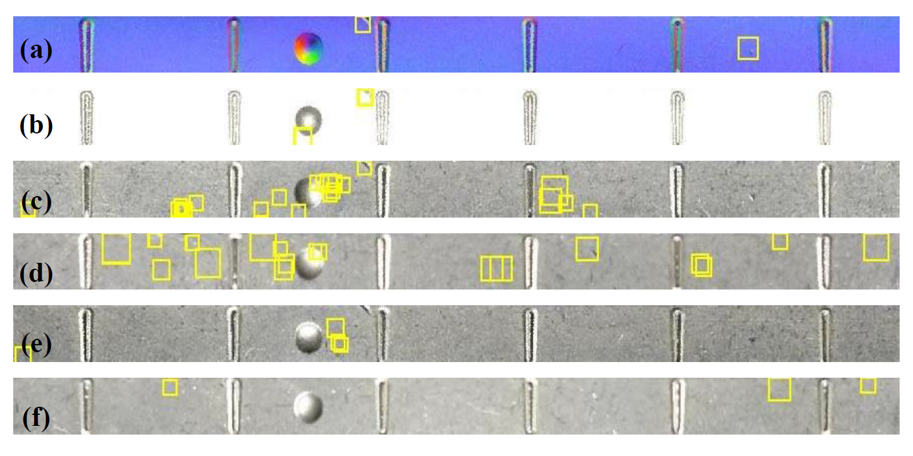
\includegraphics[width=1.0\linewidth]{figures/chuantongjiancejieguo.png}
\caption{不同输入检测结果示意图}
\label{fig:chuantongjiancejieguo}
\end{figure}
对于本文采用的评价指标结果如表\ref{tab:butongguanzhaojiancejieguo}所示,从表中不难看出,
使用不同方向光源下的照片作为数据,得到的结果非常差,
任何一项评价指标都毫无亮点,
使用顶部灯光组照片得到的结果在$recall$,$precision$上略有起色,但仍难以达到理想效果,
而使用我们提取的法线图作为数据,可以得到比较好的结果。

\begin{table}
\centering
\begin{tabular}{cccccp{38mm}}
\toprule
\textbf{输入类型} & \textbf{REC} & \textbf{PRE} & \textbf{MDR} & \textbf{FDR}\\
\midrule
\mbox{东部灯光组} & 0.6071 & 0.2484 & 0.3929 & 0.3279\\
\mbox{西部灯光组} & 0.6249 & 0.2664 & 0.3751 & 0.3072\\
\mbox{南部灯光组} & 0.7143 & 0.3091 & 0.2857 & 0.2850\\
\mbox{北部灯光组} & 0.7428 & 0.3134 & 0.2572 & 0.2905\\
\mbox{顶部灯光组} & 0.8574 & 0.5022 & 0.1426 & 0.1517\\
\mbox{法线图} & 0.9293 & 0.5981 & 0.0707 & 0.1115\\
\bottomrule
\end{tabular}
\caption{不同光照条件下检测结果表}
\label{tab:butongguanzhaojiancejieguo}
\end{table}

接着,我们分别使用法线图的梯度特征、HOG特征、LBP特征、GLCM特征、Haar-like特征、以及本身的颜色信息作为模型的输入特征,
在7个子数据集上训练出不同的强分类器,
并使用级联的方法做检测,
实验结果如表\ref{tab:butongtezhengjieguobiao}所示,
从中不难看出,使用梯度特征、HOG特征和颜色信息$(RGB)$
得到的结果要明显好于使用LBP特征、GLCM特征和Haar-like特征得到的结果。
我们认为梯度特征、HOG特征本身能更好的反应图像中像素值的变化情况,
而在法线图中,像素值的变化反应了零件表面的高低起伏变化情况,和缺陷本身关系密切,
并且,法线图的颜色信息同样反应了零件表面的变化情况。
有趣的是,测试的时候我们发现,有时HOG特征训练出来的模型反而不如直接使用梯度信息训练的模型效果好。
我们认为,法线图本身已经可以当做一个优秀的特征了,在此基础上提取HOG特征反而可能会丢失某些信息。
在此基础上,我们使用法向图的梯度信息、HOG特征和颜色信息作为组合特征,
重新训练出一个分类模型,取得了较好的结果,其结果在表\ref{tab:butongtezhengjieguobiao}展示。

\begin{table}
\centering
\begin{tabular}{cccccp{38mm}}
\toprule
\textbf{输入类型} & \textbf{REC} & \textbf{PRE} & \textbf{MDR} & \textbf{FDR}\\
\midrule
\mbox{Haar-like} & 0.8214 & 0.4677 & 0.1786 & 0.1669\\
\mbox{LBP} & 0.8938 & 0.5374 & 0.1062 & 0.1372\\
\mbox{Gredient} & 0.9114 & 0.5727 & 0.0886 & 0.1214\\
\mbox{HOG} & 0.9642 & 0.7207 & 0.0358 & 0.0667\\
\mbox{GLCM} & 0.7866 & 0.4921 & 0.2134 & 0.1448\\
\mbox{HOG+Gredient+RGB} & 0.9915 & 0.8158 & 0.0085 & 0.0400\\
\bottomrule
\end{tabular}
\caption{不同特征检测结果表}
\label{tab:butongtezhengjieguobiao}
\end{table}

最后,我们还测试了不同分类器的检测速度,从表\ref{tab:tezhengcesudu}可以看出,
检测速度最快的特征是haar-like特征,
LBP特征比haar-like特征略慢,
其次是梯度特征,
HOG特征需要在梯度特征的基础上进一步加工,速度比梯度特征慢,但并没有慢多少,
GLCM特征速度最慢,这是由于其特征提取时间复杂度最高,
本文综合梯度信息、HOG特征和颜色信息做检测速度比HOG特征稍慢,但仍然非常快。
\begin{table}
\centering
\begin{tabular}{cccccccp{38mm}}
\toprule
\mbox{特征种类} & \mbox{Haar-like} & \mbox{LBP} & \mbox{Gredient} & \mbox{HOG} & \mbox{GLCM} & \mbox{HOG+Gredient+RGB}  \\
\mbox{检测速度} & 11ms & 17ms & 16ms & 22ms & 486ms & 25ms \\
\bottomrule
\end{tabular}
\caption{不同特征检测速度表}
\label{tab:tezhengcesudu}
\end{table}
